Qui, di seguito, viene riportata l'architettura relativa alla terza solution.

\lstinputlisting[language=C++]{solutions/s3/s3.cpp}

In particolare, nella soluzione hardware in questione, rispetto alla solution 1, è stato aggiunta la direttiva di pipeline all'interno del loop1.

Effettuando la sintesi è possibile evidenziare il seguente report:\\

\begin{table}[H]
	\centering
	\begin{minipage}[t]{0.45\linewidth}
		\centering
		\begin{tabular}{|c|c|c|c|}
			\hline
			\textbf{Clock} & \textbf{Target} & \textbf{Estimated} & \textbf{Uncertainty} \\
			\hline
			ap\_clk & 10.00 & 8.510 & 1.25 \\
			\hline
		\end{tabular}
		\caption{HLS Solution 3 Timing Summary (ns)}
		\label{tab:hls-solution-3-timing-summary}
	\end{minipage}
	\hfill
	\begin{minipage}[t]{0.45\linewidth}
		\centering
		\begin{tabular}{|c|c|c|c|}
			\hline
			\multicolumn{2}{|c|}{\textbf{Latency}} & \multicolumn{2}{|c|}{\textbf{Interval}} \\
			min & max & min & max \\
			\hline
			13 & 93 & 13 & 93 \\
			\hline
		\end{tabular}
		\caption{HLS Solution 3 Latency Summary (clock cycles)}
		\label{tab:hls-solution-3-latency-summary}
	\end{minipage}
\end{table}

\begin{table}[H]
	\centering
	\begin{tabular}{|c|c|c|c|c|c|c|c|c|}
		\hline
		\multicolumn{1}{|c|}{Loop} & \multicolumn{2}{|c|}{\textbf{Latency}} & \multicolumn{1}{c|}{\textbf{Iteration Latency}} & \multicolumn{2}{c|}{\textbf{Initiation Interval}} & \multicolumn{1}{c|}{\textbf{Trip Count}}  \\
		Name & min & max &  & achieved & target &  \\
		\hline
		- loop1 & 12 & 92 & 3$\sim$23 & - & - & 4 \\
		+ loop2 & 0 & 20 & 5 & - & - & 0$\sim$4 \\
		\hline
	\end{tabular}
	\caption{HLS Solution 3 Latency Loops Summary}
	\label{tab:hls-solution-3-loop-summary}
\end{table}

Si può notare come, in questo caso l'Initiation Interval sia non specificato nel loop2 dal momento che la direttiva introdotta nella solution 2 è stata eliminata per la soluzione hardware in questione. Molto più importante è che, considerando la direttiva di pipeline definita all'interno del loop1, in corrispondenza dell'Initiation Interval di tale ciclo non è definito alcun valore numerico. Tanto è vero che, analizzando i log della sintesi presenti nella console è possibile identificare il seguente warning.
\\
WARNING: [SCHED 204-65] Unable to satisfy pipeline directive: Loop contains subloop(s) not being unrolled or flattened.
\\
In particolare, è come se il tool non riuscisse a soddisfare la richiesta di pipeline per il loop1 effettuata tramite la direttiva proprietaria. Questo potrebbe essere giustificato dal fatto che effettivamente la scissione dell'operazione "complessa" in micro-operazioni, all'interno del ciclo in questione, non è possibile effettuarla. Infatti, si può notare come i valori di latenza siano i medesimi di quelli della solution 1. Effettivamente, si potrebbe aggiungere la direttiva di pipeline all'interno del loop2, come fatto per la solution 2, dove sono presenti la maggior parte delle operazioni. In quel caso, infatti, il tool è riuscito a scomporre in micro-operazioni e così da permettere una minore latenza dal momento che i moduli potevano essere utilizzati da dati temporalmente differenti. Quello che si può notare è che nel loop1 le operazioni risultano essere l'inizializzazione della variabile temporanea \textit{ytmp}, le operazioni interne al loop2 e la scrittura del valore di \textit{ytmp} in \textit{y}. Pertanto, le uniche operazioni complesse che potrebbero essere gestite tramite una direttiva di pipeline si trovano all'interno del loop2.

\begin{figure}[H]
	\centering
	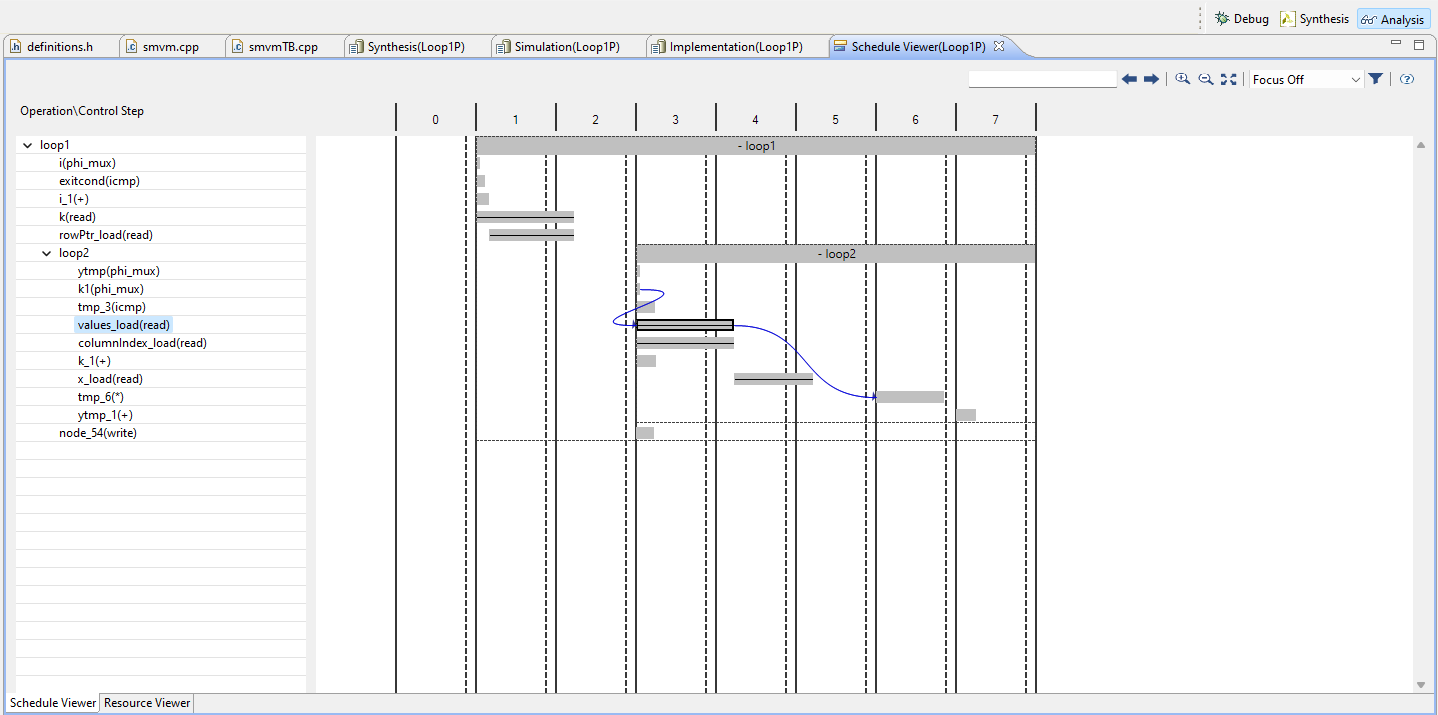
\includegraphics[width=1\textwidth]{solutions/s3/loop1pipeline.png}
	\caption{HLS Solution 3 Analysis}
\end{figure}

Qui di seguito, viene allegato l'utilizzazione delle risorse stimata dal processo di sintesi. Anche in questo caso il numero di risorse è il medesimo di quello ottenuto in corrispondenza della solution 1.
\begin{table}[h]
	\centering
	\begin{tabular}{|l|c|c|c|c|}
		\hline
		\textbf{Name}    & \textbf{BRAM\_18K} & \textbf{DSP48E} & \textbf{FF} & \textbf{LUT} \\ \hline
		DSP              & -                   & -               & -           & -            \\ 
		Expression       & -                   & 3               & 0           & 137          \\ 
		FIFO             & -                   & -               & -           & -            \\ 
		Instance         & -                   & -               & -           & -            \\ 
		Memory           & 0                   & -               & -          & -            \\ 
		Multiplexer      & -                   & -               & -           & 71          \\ 
		Register         & -                   & -               & 241         & -            \\ \hline
		\textbf{Total}   & 0                   & 3               & 241         & 208          \\ \hline
		\textbf{Available} & 280               & 220             & 106400      & 53200        \\ \hline
		\textbf{Utilization (\%)} & 0            & 1               & $\sim$0     & $\sim$0      \\ \hline
	\end{tabular}
	\caption{HLS Solution 3 Utilization Estimates Summary}
	\label{tab:hls-solution-3-utilization-estimates-summary}
\end{table}

Successivamente effettuando la C/RTL Cosimulation e l'Export RTL è possibile evidenziare i seguenti report. Anche in questo caso, sia il report del C/RTL Cosimulation sia quello dell'Export RTL risultano essere i medesimi di quelli della solution 1.
\begin{table}[H]
	\centering
	\begin{tabular}{|c|c|c|c|c|c|c|c|}
		\hline
		\multicolumn{1}{|c|}{RTL} & \multicolumn{1}{|c|}{Status} & \multicolumn{3}{c|}{\textbf{Latency}} & \multicolumn{3}{c|}{\textbf{Interval}} \\
		&  & min & avg & max & min & avg & max \\
		\hline
		VHDL & Pass & 58 & 58 & 58 & NA & NA & NA \\
		\hline
	\end{tabular}
	\caption{HLS Solution 1 with Trip Count C/RTL Cosimulation Summary }
	\label{tab:hls-solution-1-cosimulation-summary}
\end{table}

\begin{table}[H]
	\centering
	\begin{minipage}[t]{0.45\linewidth}
		\centering
		\begin{tabular}{|l|r|}
			\hline
			\textbf{Resource} & \textbf{VHDL} \\
			\hline
			SLICE & 48 \\
			\hline
			LUT & 94 \\
			\hline
			FF & 161 \\
			\hline
			DSP & 3 \\
			\hline
			BRAM & 0 \\
			\hline
			SRL & 0 \\
			\hline
		\end{tabular}
		\caption{HLS Solution 2t Export RTL Resource Usage}
		\label{tab:hls-solution-2-export-rtl-resoruce-usage}
	\end{minipage}
	\hfill
	\begin{minipage}[t]{0.45\linewidth}
		\centering
		\begin{tabular}{|l|r|}
			\hline
			\textbf{Timing} & \textbf{VHDL} \\
			\hline
			CP required & 10.000 \\
			\hline
			CP achieved post-synthesis & 5.745 \\
			\hline
			CP achieved post-implementation & 5.692 \\
			\hline
		\end{tabular}
		\caption{HLS Solution 2 Export RTL Final Timing}
		\label{tab:hls-solution-2-export-rtl-final-timing}
	\end{minipage}
\end{table}


Pertanto, considerando la solution in questione, la si potrebbe modificare aggiungendo la direttiva di pipeline anche nel loop2 per capire se le ipotesi, effettuate precedentemente, possono essere confermate o meno. 

\lstinputlisting[language=C++]{solutions/s3/s3modificata.cpp}

Adottando questo approccio, però, la nuova soluzione hardware in questione si ricondurrebbe alla solution 2 precedentemente analizzata dal momento che la direttiva di pipeline nel loop1 verrebbe comunque ignorata e quello che verrebbe effettivamente attuato sarebbe il pragma di pipeline all'interno del loop2. Infatti, effettuando la sintesi si può notare come sia presente il medeesimo warning, alleegato precedentemente, e come sia i valori di latenza sia quelli dell'utilizzazione delle risorse siano i medesimi.
\\
WARNING: [SCHED 204-65] Unable to satisfy pipeline directive: Loop contains subloop(s) not being unrolled or flattened.

\begin{table}[H]
	\centering
	\begin{minipage}[t]{0.45\linewidth}
		\centering
		\begin{tabular}{|c|c|c|c|}
			\hline
			\textbf{Clock} & \textbf{Target} & \textbf{Estimated} & \textbf{Uncertainty} \\
			\hline
			ap\_clk & 10.00 & 8.510 & 1.25 \\
			\hline
		\end{tabular}
		\caption{HLS Solution 3 Modified Timing Summary (ns)}
		\label{tab:hls-solution-3-modified-timing-summary}
	\end{minipage}
	\hfill
	\begin{minipage}[t]{0.45\linewidth}
		\centering
		\begin{tabular}{|c|c|c|c|}
			\hline
			\multicolumn{2}{|c|}{\textbf{Latency}} & \multicolumn{2}{|c|}{\textbf{Interval}} \\
			min & max & min & max \\
			\hline
			17 & 45 & 17 & 45 \\
			\hline
		\end{tabular}
		\caption{HLS Solution 3 Modified Latency Summary (clock cycles)}
		\label{tab:hls-solution-3-modified-latency-summary}
	\end{minipage}
\end{table}

\begin{table}[H]
	\centering
	\begin{tabular}{|c|c|c|c|c|c|c|c|c|}
		\hline
		\multicolumn{1}{|c|}{Loop} & \multicolumn{2}{|c|}{\textbf{Latency}} & \multicolumn{1}{c|}{\textbf{Iteration Latency}} & \multicolumn{2}{c|}{\textbf{Initiation Interval}} & \multicolumn{1}{c|}{\textbf{Trip Count}}  \\
		Name & min & max &  & achieved & target &  \\
		\hline
		- loop1 & 16 & 44 & 4$\sim$11 & - & - & 4 \\
		+ loop2 & 0 & 7 & 5 & 1 & 1 & 0$\sim$4 \\
		\hline
	\end{tabular}
	\caption{HLS Solution 3 Modified Latency Loops Summary}
	\label{tab:hls-solution-3-modified-loop-summary}
\end{table}

\begin{table}[h]
	\centering
	\begin{tabular}{|l|c|c|c|c|}
		\hline
		\textbf{Name}    & \textbf{BRAM\_18K} & \textbf{DSP48E} & \textbf{FF} & \textbf{LUT} \\ \hline
		DSP              & -                   & -               & -           & -            \\ 
		Expression       & -                   & 3               & 0           & 141          \\ 
		FIFO             & -                   & -               & -           & -            \\ 
		Instance         & -                   & -               & -           & -            \\ 
		Memory           & 0                   & -               & -          & -            \\ 
		Multiplexer      & -                   & -               & -           & 78          \\ 
		Register         & -                   & -               & 340         & 32            \\ \hline
		\textbf{Total}   & 0                   & 3               & 340         & 251          \\ \hline
		\textbf{Available} & 280               & 220             & 106400      & 53200        \\ \hline
		\textbf{Utilization (\%)} & 0            & 1               & $\sim$0     & $\sim$0      \\ \hline
	\end{tabular}
	\caption{HLS Solution 3 Modified Utilization Estimates Summary}
	\label{tab:hls-solution-3-modified-utilization-estimates-summary}
\end{table}

